%A Contratação Pública em Portugal pode ser classificada de duas formas: aberta e fechada. As regras presentes no Código dos Contratos Públicos (CCP) dizem respeito aos contratos públicos celebrados entre uma entidade adjudicante pública e uma entidade adjudicatária.

%sendo esta composta por atos e formalidades relativos à formação, conclusão e produção de uma plena eficácia jurídica de um contrato público. A eficácia jurídica - ao contrário da eficácia social - é um conceito teórico, segundo o qual uma norma definida de acordo com a lei se torna eficaz em termos jurídicos. \\

%O ato de adjudicar consiste em conferir o direito de algo a alguém, conceder algo ao maior licitante ou atribuir algo a alguém por concurso ou por ajuste. 
%Este é um termo essencial na área de contratação pública, sendo esta constituída pelas entidades adjudicantes e entidades adjudicatárias. 

%O CCP é aplicado a entidades adjudicantes públicas, tais como o Estado, Regiões Autónomas, Autarquias locais, Institutos públicos, Entidades Administrativas Independentes, Banco de Portugal, Fundações Públicas, Associações Públicas, Associações de que façam parte uma ou várias pessoas coletivas referidas anteriormente e que sejam maioritariamente financiadas por estas. Além destas, são consideradas entidades adjudicantes organismos de direito público, pessoas coletivas e associações \footnote{nos termos do artigo 2.º n.º 2, alíneas a), b) e d)}. São consideradas, também, entidades adjudicantes organismos com atuação nos setores especiais da água, energia, tranposrtes e serviços postais \footnote{artigo 7.º n.º 1.º}. Existe, também, a possibilidade de aplicar o CCP a entidades não adjudicantes que pretendem celebrar determinados contratos de empreitadas de obras públicas ou de serviços associados a obras \footnote{artigo 275.º}.


% Associações de que façam parte uma ou várias pessoas coletivas referidas anteriormente, desde que sejam maioritariamente financiadas por estas, estejam sujeitas ao seu controle de gestão ou tenham um órgão de administração, de direção ou de fiscalização cuja maioria dos titulares seja, direta ou indiretamente, designada pelas mesmas

% São ainda entidades adjudicantes organismos de direito público, pessoas coletivas e associações, independentemente da sua natureza pública ou privada, nos termos do artigo 2.º n.º 2, alíneas a), b) e d).

% Para além das entidades adjudicantes referidas no artigo 2º, são também entidades adjudicantes as referidas no artigo 7.º n.º 1.º, concretamente as pessoas coletivas que realizam atividades nos seguintes sectores especiais da água, energia, transportes e serviços postais.

% O CCP aplica-se ainda a entidades que não sendo adjudicantes, se encontrem nas situações previstas no artigo 275.º, ou seja, entidades que pretendam celebrar determinados contratos de empreitadas de obras públicas ou de serviços associados a obras, desde que estes contratos sejam subsidiados diretamente em mais de 50\% do respetivo preço contratual por entidades adjudicantes, sempre que o preço contratual for igual ou superior aos limiares comunitários.


%Existem duas fases principais no processo de contratação pública. 
%A primeira fase é a \textbf{fase preparatória} em que é feita a decisão de realizar um contrato e inclui uma fase preparatória do procedimento e uma fase instrutória que terminará no ato de ajudicação. A segunda fase é a \textbf{fase conclusiva} em que é concluído e celebrado o contrato. Existe também uma \textbf{fase complementar} que pode ser necessária na eventualidade do contrato público depender de atos posterioes à sua celebração tais como a aprovação, visto e publicidade. \\

\section{Código dos Contratos Públicos}

O Código dos Contratos Públicos (CCP) é um documento que estabelece um alinhamento com as mais recentes diretivas comunitárias,  estabelecidas pelo Parlamento Europeu \cite{ue_dire}, definindo um conjunto homogéneo de normas relativas aos processos pré-contratuais e uma nova sistematização e uniformização de regimes substantivos dos contratos administrativos. 

Este encontra-se dividido em duas grandes categorias: \textbf{disciplina aplicável à contratação pública} e \textbf{regime substantivo dos contratos públicos}, correspondentes às Partes II e III do documento, respetivamente.

O CCP pauta-se por um conjunto de objetivos gerais que podem ser observados na figura \ref{fig:ccpgoals}.

\begin{figure}[H]
	\centering
	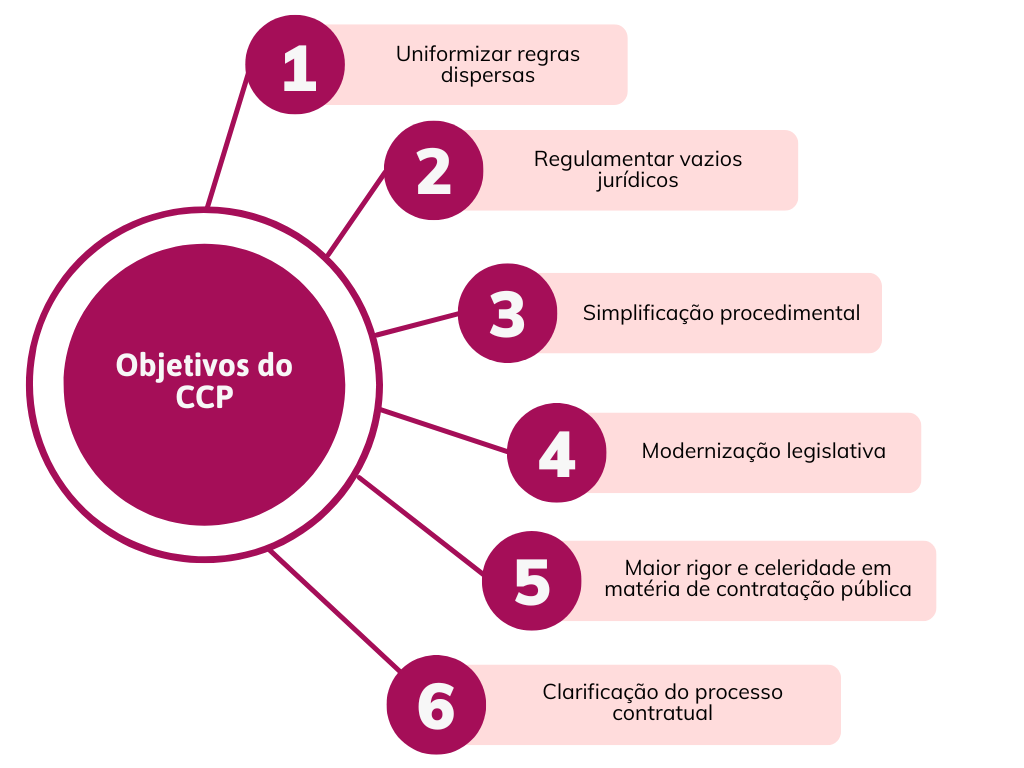
\includegraphics[width=0.7\textwidth]{imagens/ccp_objetivos.png}
	\caption{Objetivos Gerais do Código dos Contratos Públicos}
	\label{fig:ccpgoals}
\end{figure}


Pretende-se simplificar a tramitação procedimental pré-contratual através de novas tecnologias de informação/meios eletrónicos, incentivando a desburocratização, a desmaterialização, criando sistemas alternativos à utilização de papel, e a simplificação da contratação pública. 


Ao longo do processo contratual são definidas vários requisitos que devem ser cumpridos.
Relativamente ao \textbf{nível de qualificação dos candidatos}, é exigido que os mesmos demonstrem que possuem tanto capacidade técnica como financeira a fim de completar o objeto contratual. 

É imperativo que os \textbf{métodos de avalição de propostas}, componente crucial na formação e celebração de contratos públicos, sejam devidamente enunciados e publicitados, de modo a que as entidades concorrentes desenvolvam uma estratégia/proposta eficiente e a entidade adjudicante escolha, à luz desses mesmos critérios, a proposta mais vantajosa a nível económico na ótica do interesse prosseguido. 

Além do mais, o CCP procura, de forma cabal, garantir que a enunciação e publicitação dos critérios de adjudicação e respetivos coeficientes de ponderação se faça em moldes conformes com os princípos da igualdade, da concorrência, da imparcialidade, da proporcionalidade, da transparência, da publicidade e da boa fé. 




É, também, desejável que o objeto do contrato a celebrar \textbf{reflita e valorize preocupações de cariz social e ambiental}. 

O incumprimento da legislação pode levar a correções financeiras, cujas taxas são definidas em função da natureza e gravidade das irregularidades em causa e, consequentemente, a uma perda de financiamento. As irregularidades que são detetadas com maior frequência encontram-se disponíveis para consulta na Tabela COCOF \cite{corrections}.

\subsection{Entidades}

O artigo 2.º do CCP categoriza as entidades adjudicantes em dois organismos: Organismos pertencentes ao setor público administrativo tradicional e Organismos de direito público.


\begin{table}[h!]
	
	\centering
	\setlength{\tabcolsep}{15pt}
	\setlength\cellspacetoplimit{0.5cm} 
	\setlength\cellspacebottomlimit{0.5cm} 
	\renewcommand{\arraystretch}{1.5}

	\resizebox{\textwidth}{!}{
        \begin{tabular}{p{0.1\textwidth} p{0.1\textwidth} p{0.1\textwidth} p{0.25\textwidth} m{0.5\textwidth}} % Use p{} column type for vertical padding

			\hline
			\multicolumn{5}{Sc}{\textbf{Entidades Adjudicantes}} \\
			\hline
			\rowcolor[HTML]{EFEFEF} 
			\multicolumn{4}{Sc|}{\cellcolor[HTML]{EFEFEF}\textbf{Organismos pertencentes ao setor público administrativo tradicional}} & \textbf{Organismos de direito público} \\
			\hline
			Estado & Regiões Autónomas & Autarquias locais & Institutos públicos & \multirow{2}{=}{\centering Quaisquer pessoas coletivas que, independentemente da sua natureza pública ou privada, reúnam os requisitos presentes no n.º2 do artigo 2.º} \\ 
			Banco de Portugal & Fundações Públicas & Associações públicas & Entidades administrativas independentes & \\
			\hline
		\end{tabular}
	}
	
	\caption{Categorização das Entidades Adjudicantes}
	\label{table:1}
\end{table}



Existem, além das já mencionadas, outro tipo de entidades adjudicantes, também abrangidas pelo CCP, pertencentes aos setores especiais da água, energia, transportes e serviços postais. 

É de salientar que a denominação  de \textit{entidade adjudicante} apenas é válida durante a fase pré-contratual. Após a celebração do contrato, passa a ser denominada como \textit{contraente público}. 



\subsection{Procedimentos para formação de contratos}
%\subsubsection{Equadramento Legal}

\subsubsection{Tipos de Procedimento e Contrato}
Os procedimentos pré-contratuais definidos no n.º1 do artigo 16.º, a serem adotados pelas entidades adjudicantes, encontram-se na Tabela \ref{table:2}.

\begin{table}[ht]
	\centering
	\renewcommand{\arraystretch}{1.15}
	\setlength{\tabcolsep}{15pt}
	%\resizebox{\textwidth}{!}{%
		\begin{tabular}{lc}
			\toprule
			\multicolumn{1}{c}{\textbf{Tipo de Procedimento}} & \textbf{Artigo do CCP} \\ 
			\midrule
			\rowcolor[HTML]{EFEFEF} 
			Ajuste Direto                                     & 112.º a 129.º          \\ 
			Consulta Prévia                                   & 112.º a 127.º          \\
			\rowcolor[HTML]{EFEFEF} 
			Concurso Público                                  & 130.º a 161.º          \\
			Concurso Limitado por Prévia Qualificação         & 162.º a 192.º          \\
			\rowcolor[HTML]{EFEFEF} 
			Diálogo Concorrencial                             & 204.º a 218.º          \\
			Procedimento de Negociação                        & 193.º a 203.º          \\
			\rowcolor[HTML]{EFEFEF} 
			Parceria para a Inovação                          & 218.º-A a 218.º-D      \\
			Acordos-quadro                                    & 251.º a 259.º          \\                             
			\bottomrule
		\end{tabular}
	%}
	\caption{Tipos de Procedimento Pré-Contratuais}
	\label{table:2}
\end{table}


\begin{my_enumerate}
	
	\item O \textbf{ajuste direto} consiste no convite, por parte da entidade adjudicante, a um operador económico à sua escolha, a fim de apresentar uma proposta para um determinado objeto contratual.
	
	\item Na \textbf{consulta prévia}, a entidade adjudicante convida diretamente, pelo menos, 3 operadores económicos à sua escolha a apresentar uma proposta. Os aspetos referentes ao contrato a celebrar podem ser negociados diretamente entre a entidade adjudicante e os operadores convidados. 
	
	\item O \textbf{concurso público} pode ser adotado sempre que uma determinada entidade adjudicante o decidir. Não existe nenhuma fase prévia de qualificação dos concorrentes relativamente à capacidade técnico-financeira. 
	
	\item O \textbf{concurso limitado por prévia qualificação} é adotado quando o valor do contrato a celebrar for superior aos limiares Europeus. Neste caso, o concurso é dado a conhecer, não só através do Diário da República, como nos itens anteriores, como no Jornal Oficial da União Europeia. O \textbf{procedimento de negociação} partilha algumas características com este procedimento. 
	
	\item O \textbf{diálogo concorrencial} é utilizado nas situações em que a entidade adjudicante identifica uma necessidade e não sabe como satisfazer. 
	
	\item A \textbf{parceria para a inovação} destina-se à realização de atividades de investigação e desenvolvimente de bens, serviços ou obras inovadoras. Tem como objetivo a aquisição destes bens desde que se cumpram os níveis de desempenho de preços máximos
	previamente combinados. Acontece quando um entidade adjudicante pretende adquirir um bem/serviço/obra
	pública com determinadas características que não se encontram no mercado. 
	
	\item O \textbf{acordo quadro} é a celebração de um contrato entre uma ou várias entidades adjudicantes e uma ou mais entidades. 
	
	
	
\end{my_enumerate}

Em ambos os casos existem limitações relativamente aos operadores económicos que podem ser convidados. (artigos 19.o, al. d), e 20.o, n.o 1, al. d), 19.o, al. c), e 20.o, n.o 1, al. c)). Não obstante, as limitações referidas não se aplicam em contratos ao abrigo de critérios materiais. 
A celebração de consultas prévias e ajustes diretos deve ser publicitada no Portal dos Contratos Públicos pela entidade ajdudicante no prazo máximo de 20 dias a contar da data de celebração do contrato, a fim de comprovar a eficácia do respetivo contrato. 



%\textit{O CCP revê em alta ( o que é que isto significa? ) os limites relativos ao valor do contrato em função do procedimento pré-contratual adoptado. Para efeitos da determinação do valor do contrato, foi estabelecido que a escolha do procedimento condiciona o valor do contrato a celebrar. Por sua vez, o valor do contrato a celebrar pode ser entendido como o valor máximo do benefício económico obtido pelo adjudicatário com a execução de todas as prestações que constituem o objeto contratual.} \\



O n.º2 do mesmo artigo designa a tipologia do contrato a realizar, independentemente da sua natureza ou designação. 

\begin{table}[h!]
	\centering
	\renewcommand{\arraystretch}{1.15}
	\setlength{\tabcolsep}{15pt}
	%\resizebox{\textwidth}{!}{%
		\begin{tabular}{lc}
			\toprule
			\multicolumn{2}{c}{\textbf{Tipo de Contrato}}                                              \\ 
			\midrule
			Empreitada de obras públicas   &                                   \\
			Concessão de obras públicas                            & \multirow{-2}{*}{Obras}           \\ \hline
			Concessão de serviços públicos &                                   \\
			Locação ou aquisição de bens móveis                    &                                   \\
			Aquisição de serviços          &                                   \\
			Sociedade                                              & \multirow{-4}{*}{Bens e Serviços} \\ 
			\bottomrule
		\end{tabular}%
		%}
	\caption{Tipos de Contrato}
	\label{table:3}
\end{table}

FALAR DAS TIPOLOGIAS DE FORMA BREVE

\begin{figure}[H]
	\centering
	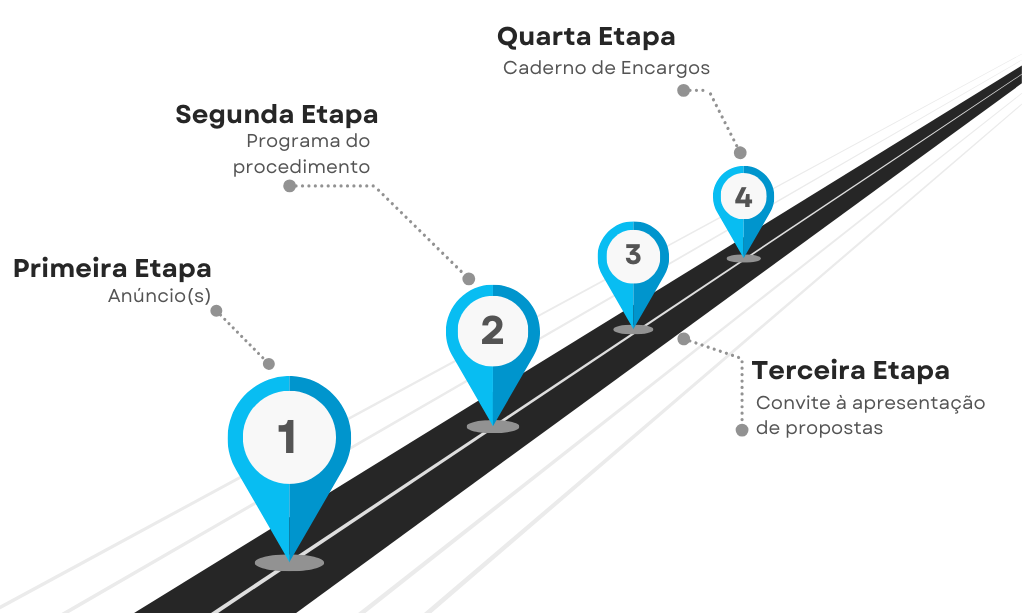
\includegraphics[width=0.75\textwidth]{imagens/pecasprocedimento.png}
	\caption{Peças do Procedimento}
	\label{fig:pecas}
\end{figure}

Na figura \ref{fig:pecas} é possível visualizar, de uma forma simplista, as peças que são transversais a todos os tipos de procedimento. \footnote{No caso do Ajuste Direto e Consulta Prévia não são tidas em conta as duas primeiras etapas. No Diálogo Concorrencial existem outras etapas intermédias.} 
São estas peças que definem as formalidades e requisitos que devem cumpridos na fase de elaboração e apresentação de propostas pelas entidades concorrentes. 
O anúncio do concurso público é sempre feito no Diário da República e, sob determinadas circunstâncias, no Jornal Oficial da União Europeia. 
O programa do procedimento é o regulamento que define os termos que devem ser cumpridos desde a fase de formação do contrato até ao seu término \cite{programaproc}. 
Por sua vez, o caderno de encargos é a peça do procedimento onde estão definidas as cláusulas do contrato a celebrar \cite{caderno}. 


\subsubsection{Escolha do procedimento}

O artigo 36.º do CCP define que a escolha do tipo de procedimento aquando da decisão de contratar deve ser fundamentada. Antes da abertura de um procedimento de formação de contrato público, a entidade adjudicante pode efetuar consultas informais de mercado a serem, eventualmente, usadas no planeamento da contratação. No caso de essa consulta ser feita a uma empresa que, posteriormente, se candidate ao concurso em questão, deve ser comunicado essa informação aos restantes concorrentes e inclui-la nas peças do procedimento. 

Além do mais, aquando da escolha do tipo de procedimento, devem ser tidas em conta as duas possíveis modalidades: \textbf{Critério do Valor} e \textbf{Critério Material}. 
Se se optar pelo critério do valor, existem valores máximos tabelados para o valor que o contrato pode tomar, consoante o tipo de procedimento. Define-se como valor do contrato o valor máximo do benefício económico obtido pela entidade contratada após a completitude de todas as prestações pertencentes ao objeto contratual.


\begin{table}[h!]
	\centering
	\renewcommand{\arraystretch}{1.6}
	\setlength{\tabcolsep}{15pt}
	\resizebox{\textwidth}{!}{%
		\begin{tabular}{ccccc}
			\hline
			\multicolumn{2}{c}{\textbf{Tipo de Procedimento}}                     & \textbf{Preço Base}                        & \textbf{Objeto} & \textbf{Base Legal (CCP)} \\ \hline
			\multirow{5}{*}{Ajuste Direto} & \multirow{2}{*}{Regime Simplificado} & \textless{}= €10.000,00                    & Obras           & artigo 128.º, n.º1        \\
			&                                      & \textless{}= €5.000,00                     & Bens e Serviços & artigo 128.º, n.º1        \\
			& \multirow{3}{*}{Regime Geral}        & \textless{}= €30.000,00                    & Obras           & artigo 19.º, al d)        \\
			&                                      & \textless{}= €20.000,00                    & Bens e Serviços & artigo 20.º, n.º1, al c)  \\
			&                                      & \textless{}= €50.000                       & Outros          & artigo 21.º, n.º1, al c)  \\ \hline
			\multicolumn{2}{c}{\multirow{3}{*}{Consulta Prévia}}                  & \textless{}= €150.000,00                   & Obras           & artigo 19.º, al c)        \\
			\multicolumn{2}{c}{}                                                  & \textless{}= €75.000,00                    & Bens e Serviços & artigo 20.º, n.º1, al c)  \\
			\multicolumn{2}{c}{}                                                  & \textless{}= €100.000                      & Outros          & artigo 21.º, n.º1, al c)  \\ \hline
			\multicolumn{2}{c}{\multirow{3}{*}{Concurso Público}}                 & \multirow{2}{*}{Até aos Limiares Europeus} & Obras           & artigo 19.º, al b)        \\
			\multicolumn{2}{c}{}                                                  &                                            & Bens e Serviços & artigo 20.º, n.º1, al b)  \\
			\multicolumn{2}{c}{}                                                  & Qualquer valor                             & Outros          & artigo 21.º, n.º1, al a)  \\ \hline
		\end{tabular}%
	}
	\caption{Valores máximos por tipo de procedimento}
	\label{tab:4}
\end{table}



Se for elegido o \textbf{Critério do Valor} é permitida a celebração de contratos de qualquer valor (de acordo com o artigo n.º23). Para tal, é necessário que o órgão competente para a decisão de contratar fundamente, de forma clara e objetiva, que a situação cumpre todos os requisitos previstos (nos artigos n.º24 a n.º27).


\subsubsection{Tipos de Contratos}

Os \textbf{contratos mistos} consistem num objeto contratual que contempla a prestação de dois ou mais tipos de contrato diferentes (nr.º1 do artigo 32.º). Por exemplo, o fornecimento de bens móveis e a prstação de serviços.

A \textbf{adjudicação por lotes} consiste na divisão de um contrato avultado em vários contratos de dimensão inferior, sendo o número máximo de lotes definido pela entidade adjudicante. Desta forma, é permitida a participação de pequenas e médias empresas que não teriam capacidade organizacional e técnico-financeira adequada para a realização total do contrato. 

\begin{table}[h!]
	\centering
	\renewcommand{\arraystretch}{1.45}
	\setlength{\tabcolsep}{15pt}
	\begin{tabular}{cc}
		\hline
		\textbf{Tipo de Contrato} & \textbf{Valor Mínimo} \\ \hline
		Bens e Serviços           & €135.000,00           \\
		Empreitadas               & €500.000,00           \\ \hline
	\end{tabular}
	\caption{Valor mínimo para Adjudicação por Lotes}
	\label{tab:5}
\end{table}

Contudo, em situações cujo preço do contrato a celebrar seja superior aos valores mínimos apresentados na tabela \ref{tab:5}, a adjudicação por lotes não é de cariz obrigatório. Carece, no entanto, de uma obrigação de fundamentação (nr.º2 do artigo 46.º-A). 


\subsection{Tramitação Procedimental}




\begin{figure}[H]
	\centering
	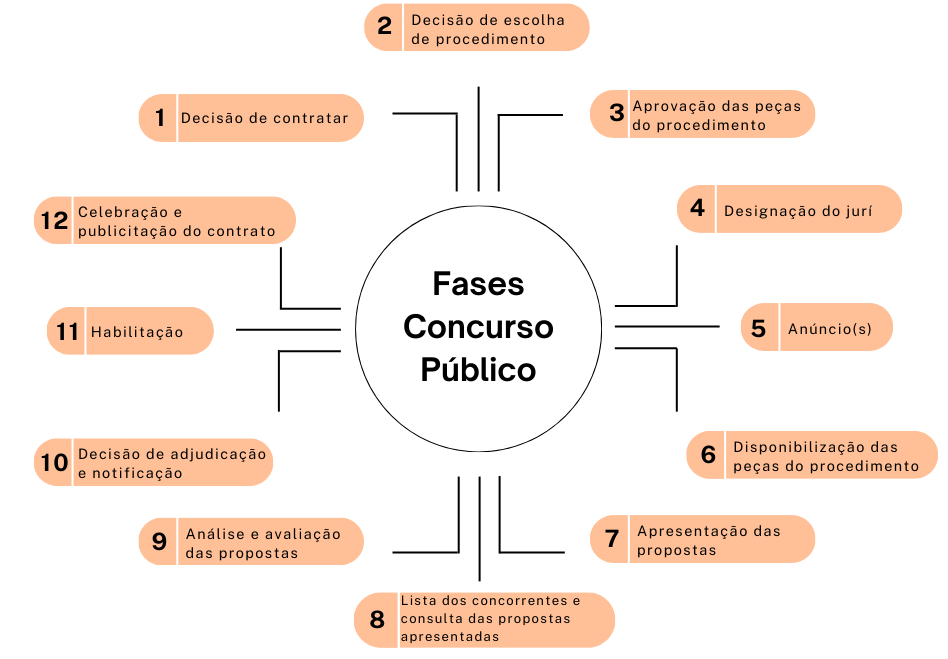
\includegraphics[width=\textwidth]{imagens/fasesconcpub.png}
	\caption{}
	\label{}
\end{figure}
